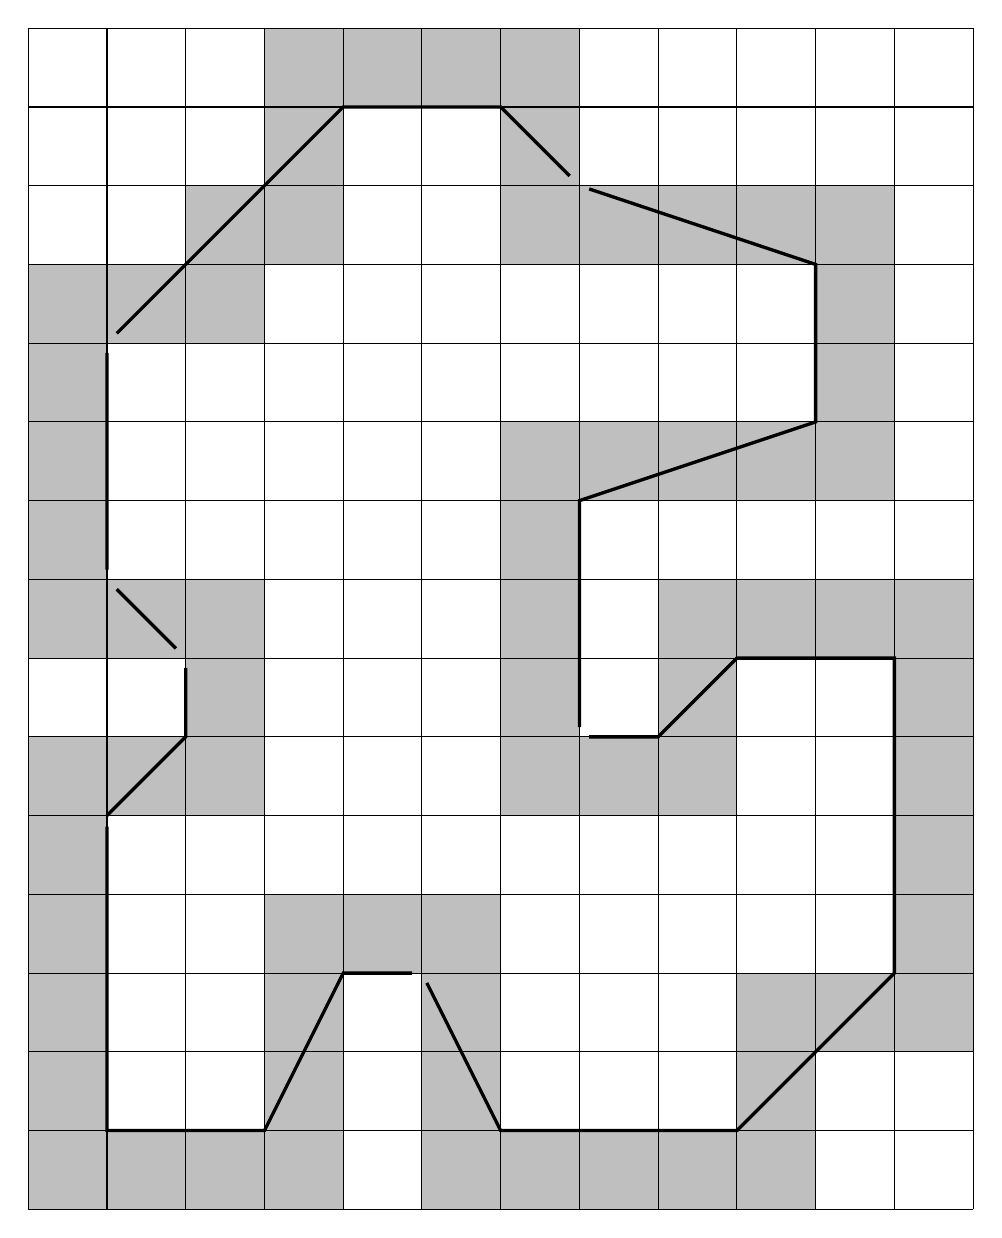
\begin{tikzpicture}

\draw [fill=lightgray] (0,12) rectangle (1,7)
 (1,8) node (v2) {} rectangle (3,7)
  (3,5) rectangle (2,7) node (v1) {}
  (2,5) rectangle (0,6)
  (0,5) rectangle (1,0)
  (1,0) rectangle (4,1)
  (4,1) rectangle (3,4)
  (4,4) rectangle (6,3)
  (5,3) node (v6) {} rectangle (6,0)
  (6,0) rectangle (10,1)
  (10,1) rectangle (9,3)
  (10,3) rectangle (12,2)
  (12,3) rectangle (11,8)
  (11,8) rectangle (8,7)
  (8,7) rectangle (9,5)
  (8,5) rectangle (6,6)
  (7,6) node (v5) {} rectangle (6,10)
  (7,10) rectangle (11,9)
 (11,10) rectangle (10,13)
  (10,13) rectangle (6,12)
  (7,13) node (v4) {} rectangle (6,15)
  (6,15) rectangle (3,14)
  (3,14) rectangle (4,12)
  (2,13) rectangle (3,11)
  (2,12) rectangle (1,11) node (v3) {};
  
 %\draw [very thick] plot[smooth, tension=.7] coordinates {(3.5,14.4) (6.5,14.3) (6.4,12.5) (9.9,12.5) (10.4,9.4) (6.8,9.5) (6.5,5.9) (8.6,5.5) (8.7,7.4) (11.4,7.3) (11.5,2.8) (9.4,2.4) (9.6,0.5) (7.1,0.4) (6.5,0.7) (5.7,0.4) (5.6,3.4) (4.6,3.3) (3.5,3.6) (3.4,0.6) (0.6,0.9) (0.7,5.5) (2.3,5.6) (2.5,7.7) (0.6,7.5) (0.4,11.4) (2.3,11.7) (2.5,12.3) (3.5,12.7) (3.4,13.3) (3.5,14.4)};

\foreach \x in {0,...,12} {
	\draw (\x,0) -- (\x,15);
}
\foreach \y in {0,...,15} {
	\draw (0,\y) -- (12,\y);
}

\draw [very thick] (1,5) node (v7) {} -- (2,6) -- (v1) -- (v2) -- (v3) -- (4,14) -- (6,14) -- (v4) -- (10,12) -- (10,10) -- (7,9) -- (v5) -- (8,6) -- (9,7) -- (11,7) -- (11,3) -- (9,1) -- (6,1) -- (v6) -- (4,3) -- (3,1) -- (1,1) -- (v7);
\end{tikzpicture}